\documentclass[conference]{IEEEtran}

\usepackage{amsmath,amssymb,amsfonts}
\usepackage{algorithmic}
\usepackage{graphicx}
\usepackage{textcomp}
\usepackage{xcolor}
\usepackage[backend=biber,style=numeric]{biblatex}

\graphicspath{{assets/latex/latex/}}

\begin{document}

\title{CS6524 Computer Vision Lab. 1\\ Silhouettes and Fourier Epicycles}

\author{\IEEEauthorblockN{1\textsuperscript{st} Frederick Sheppard}
\IEEEauthorblockA{\textit{23361433} \\
\textit{4th Year ISE}}
\and
\IEEEauthorblockN{2\textsuperscript{nd} Oluwajomiloju Olajitan}
\IEEEauthorblockA{\textit{23373326} \\
\textit{4th Year ISE}}
\and
\IEEEauthorblockN{3\textsuperscript{rd} Naem Haq}
\IEEEauthorblockA{\textit{23379243} \\
\textit{4th Year ISE}}
}

\maketitle

\begin{abstract}
We discuss a pipeline we implemented that takes an image, applies several filters and pre-processing steps to convert it into an outline, turns that outline into a one dimensional signal, uses the Fourier transform to break that signal into its harmonics, and reconstructs the signal using a configurable number of those harmonics. Parameters are set for each image to achieve the best results and an mp4 video is created showing the harmonics tracing the path of the outline. We discuss our implementation, justify our approach, and discuss the strengths, weaknesses, and future work of the project. Learning outcomes included how to break a signal into its constituent parts, how to use filters to improve the performance of image processing algorithms, and how to convert 2D data into a one dimensional signal. With more work, we could improve the effectiveness of the project, letting it generalise to a wider variety of images.
\end{abstract}




\section{Methodology}\label{sec:methodology}

\subsection{Silhouette Extraction}
We reduce each RGB image to a single channel using Rec.~601 luma or the minimum RGB value, depending on which separates
the subject from the background. For example, the orange has at least one
weak channel, so its minimum RGB value is low, whereas the white background
and the grey soft shadow remain bright in every channel. We
convolve the selected channel with a normalized Gaussian kernel extending
to $\lceil 3\sigma\rceil$ pixels on each side. Smoothing reduces small
intensity variations before segmentation. We use Otsu's threshold when no
fixed threshold is specified and select the darker or brighter side of
the threshold according to the image configuration.

Disk-shaped opening removes small foreground regions, and closing fills
small gaps. We keep the largest connected components and optionally fill
holes. The scissors example retains two components and preserves the
handle holes. To extract the inner boundary, we convolve the mask with a
four-neighbour Laplacian and retain foreground pixels with a positive
response. These pixels have at least one background neighbour. Zero
padding allows the boundary to follow the image edge where the subject
touches the frame.

\subsection{Contour Tracing and Resampling}
We discard boundary components with fewer than 20 pixels and order the
remaining pixels using Moore-neighbour tracing. When there are multiple
loops, we join them at the closest pair of points and traverse each bridge
in both directions to form a single closed path. We compute cumulative
Euclidean distance along the path and linearly interpolate the coordinates
at equally spaced arc lengths. The default is $N=500$ samples, with
$N=1000$ for the scissors. We omit the duplicated endpoint so that the
samples cover one period.

\subsection{Fourier Reconstruction}
We encode the samples as $z[n]=x[n]+\mathrm{i}y[n]$ and compute their
discrete Fourier transform $Z[k]$ using the FFT. The DC coefficient
positions the silhouette, so we always retain it and rank the remaining
coefficients by magnitude. For a reconstruction with $K$ coefficients,
let $S_K$ contain the DC index and the indices of the $K-1$ largest
remaining coefficients by magnitude.
We zero the coefficients outside $S_K$ and apply the inverse FFT,
\begin{equation}
\hat{z}_K[n] = \frac{1}{N}\sum_{k\in S_K} Z[k]
    \exp\!\left(\frac{2\pi\mathrm{i}kn}{N}\right).
\end{equation}
Each retained coefficient corresponds to a rotating vector with radius
$|Z[k]|/N$ and initial phase $\arg Z[k]$. We plot 20 reconstructions,
increasing $K$ from 5\% to 100\% of $N$ in steps of five percentage points.

Figure~\ref{fig:02_transforms} shows the complete image transformation pipeline.

\begin{figure}
    \centering
    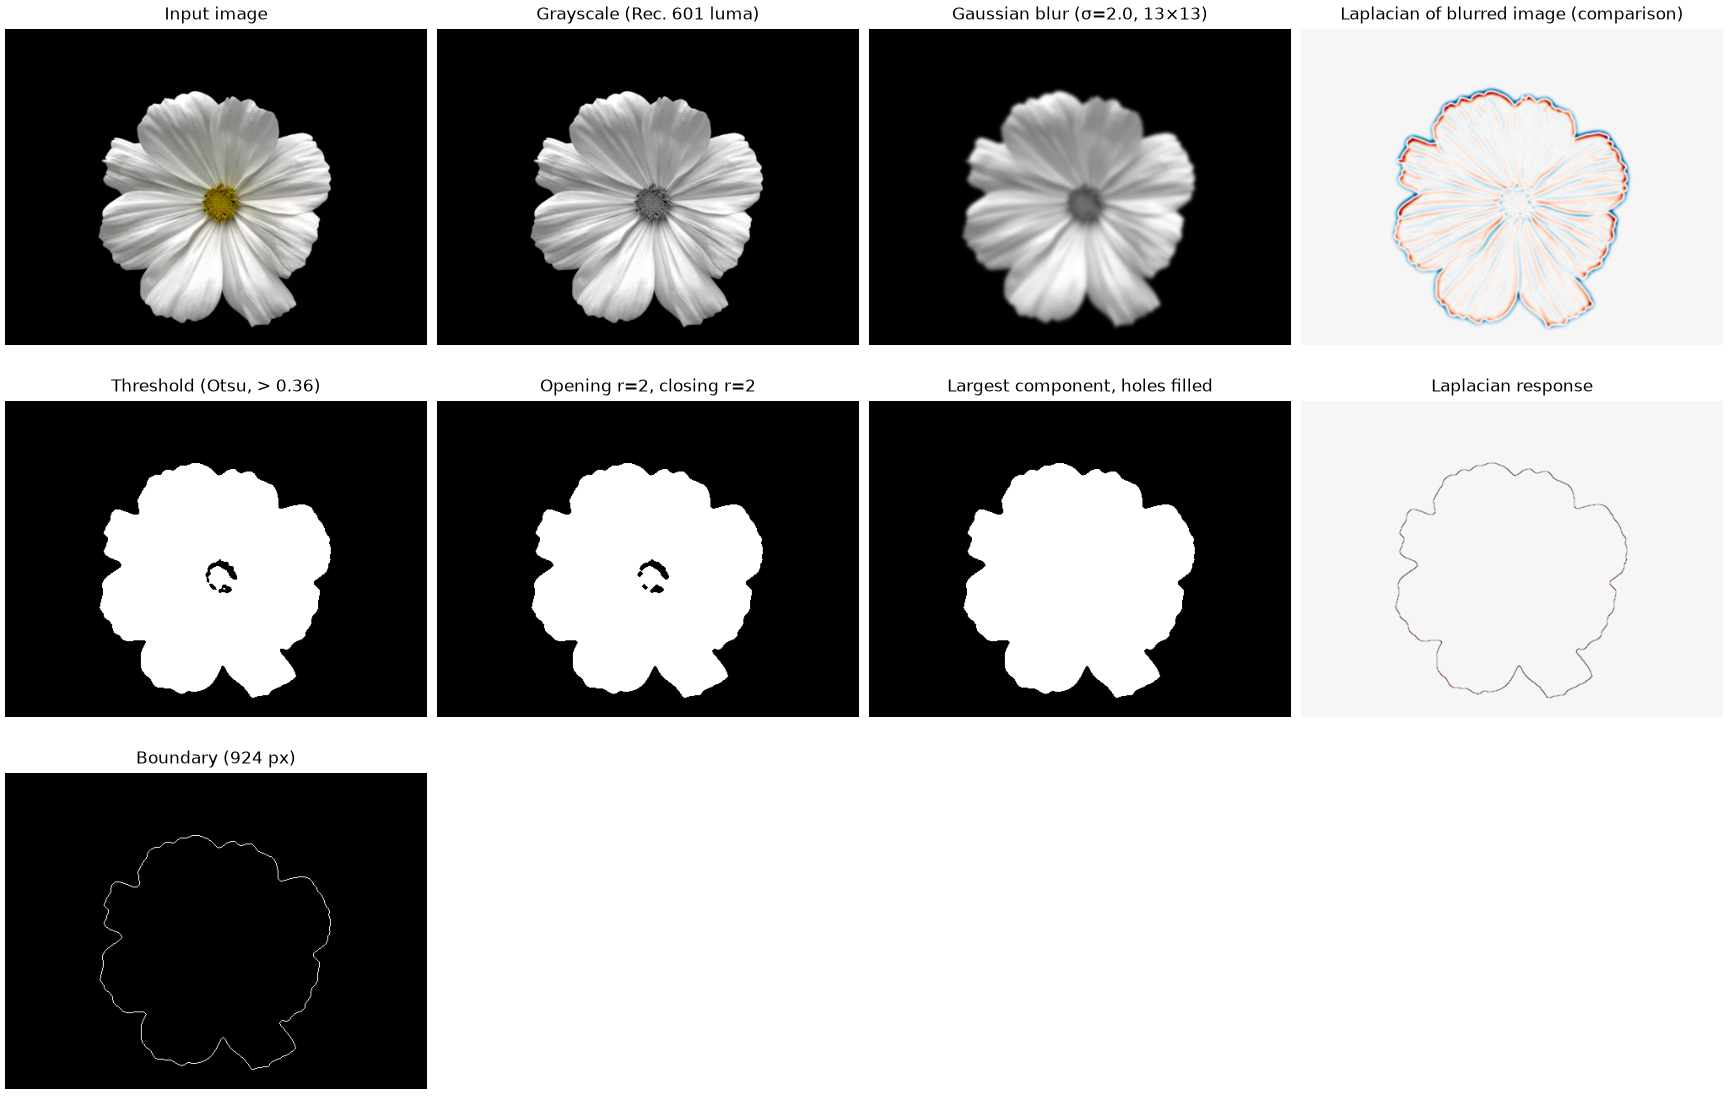
\includegraphics[width=0.5\linewidth]{assets/latex/02_transforms.png}
    \caption{Image showing the transforms applied to Image 02}
    \label{fig:02_transforms}
\end{figure}

\section{Justifications}
\label{sec:justifications}
No single parameter setting segmented all five images, so we record
image-specific settings in \texttt{in/XX.yaml}.

\subsection{Channel selection}
We compare channels using Otsu separability, the ratio of between-class
variance to total variance at the Otsu threshold. The orange peel has low
blue intensity, while the background and shadow are brighter in that
channel. Separability increases from 0.835 with luma to 0.932 with blue.
In the person image, the clothing has at least one low RGB channel, while
the grey background stays relatively bright across all three. Taking the
minimum RGB value increases separability from 0.911 to 0.939. For the
flower, succulent, and scissors, the scores differ by less than 0.01,
so we use luma.

\subsection{Gaussian smoothing}
Surface texture can produce speckles and holes after thresholding.
Increasing $\sigma$ from 0.5 to 1.5 reduces the number of holes in the
person mask from 85 to 2. For the succulent, smoothing with $\sigma=1$
reduces the mask from 18 regions and 158 holes to 8 regions and 19 holes.
Stronger smoothing erodes the thin leaf tips. We also use $\sigma=1$ for
the scissors to preserve sharp corners.

\subsection{Thresholding}
Otsu's method separates intensities by maximizing between-class variance.
Its threshold can cut through the subject when some foreground pixels
have intensities similar to the background, as with the pale orange pith
and the person's light clothing. We use fixed thresholds of 0.76, 0.08,
and 0.72 for the orange, succulent, and person, respectively, compared
with Otsu thresholds of 0.60, 0.40, and 0.51. The resulting mask areas
increase from 19,298 to 21,822 pixels, from 23,614 to 41,003 pixels, and
from 80,111 to 88,250 pixels, respectively. The flower and scissors use
Otsu thresholds of 0.36 and 0.48.

\subsection{Mask cleanup}
We implement erosion and dilation by convolving the binary mask with a
disk-shaped kernel and thresholding the response. A disk reduces the
directional bias of a square kernel. Larger radii remove more noise but
can also erase thin features, so we keep the radii small. For the
succulent, keeping the largest connected component and applying opening
with $r=1$ and closing with $r=2$ reduces the boundary from 2,137 to
1,798 pixels. For the scissors, we keep two connected components and
preserve the holes because both pairs and their handle openings are
part of the silhouette.

\subsection{Boundary extraction}
Applying the Laplacian to the blurred image also highlights internal
features such as the orange segments, succulent stripes, and clothing
folds. Applying it to the binary mask restricts the response to
transitions between foreground and background. We retain the positive
responses inside the mask to obtain a thin inner boundary for
8-neighbour contour tracing. Zero padding closes the boundary along the
frame where the scissors extend beyond the image.

\section{Discussion \& Failure Analysis}



\subsection{Implementation Strengths}

Our implementation has several pieces of evidence that stand to its strength. First, the Fourier transform implementation is measurably accurate. When using 100\% of the harmonics, reconstruction error compared to the original is around $1 \times 10^{-13}$. This means that a reconstruction is indistinguishable from the original outline. Second, the upper bound on the efficacy of our filter algorithms is very good. For image 02, the flower, only $\sigma$ had to be manually calibrated to ensure a good output, with Otsu able to select the rest automatically. This shows that the pipeline is capable of acting on some unseen images with little to no manual intervention. Finally, multi-loop handling allows more images to be rendered than would otherwise be possible. Image 04, the scissors, has loops in the handles that require special handling, as described in Section~\ref{sec:methodology}. The output shows multiple loops inside the handle, with a small bridge joining them to the main outline, showing that the technique works.

\subsection{Areas for Improvement}

There are some areas in which our implementation falls short. While multi-loop handling does allow loops to be supported, the scissors example runs into issues when the inner loop is near the boundary of the image. Three of the four loops are rendered correctly, but one is excluded (Figure~\ref{fig:04_trajectory}). Additionally, Image 3 runs into issues with the white shoe on a white background (Figure~\ref{fig:03_transforms}). Increasing the threshold value starts including the girl's shadow, making it impossible to pick a single value that accounts for both. Finally, the fact remains that other than for Image 02, multiple parameters had to be set by hand to achieve good performance on images. A more robust algorithm would be able to generalise more effectively, reducing the number of images that would have to be paramaterised by hand.

\begin{figure}
    \centering
    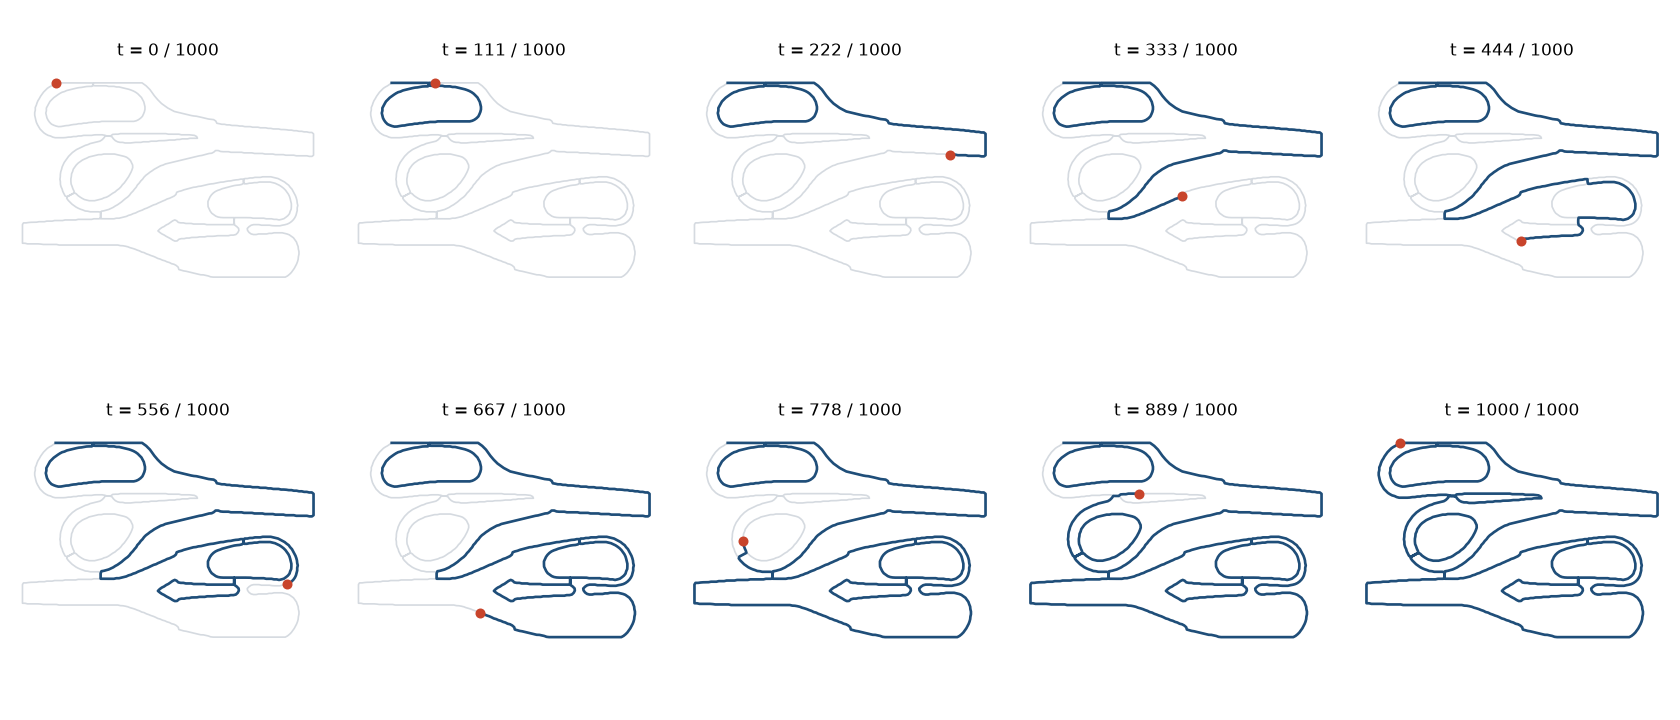
\includegraphics[width=0.5\linewidth]{assets/latex/04_trajectory.png}
    \caption{Image showing the trajectory of tracing Image 04. Note the missing loop at near the boundary of the image.}
    \label{fig:04_trajectory}
\end{figure}

\begin{figure}
    \centering
    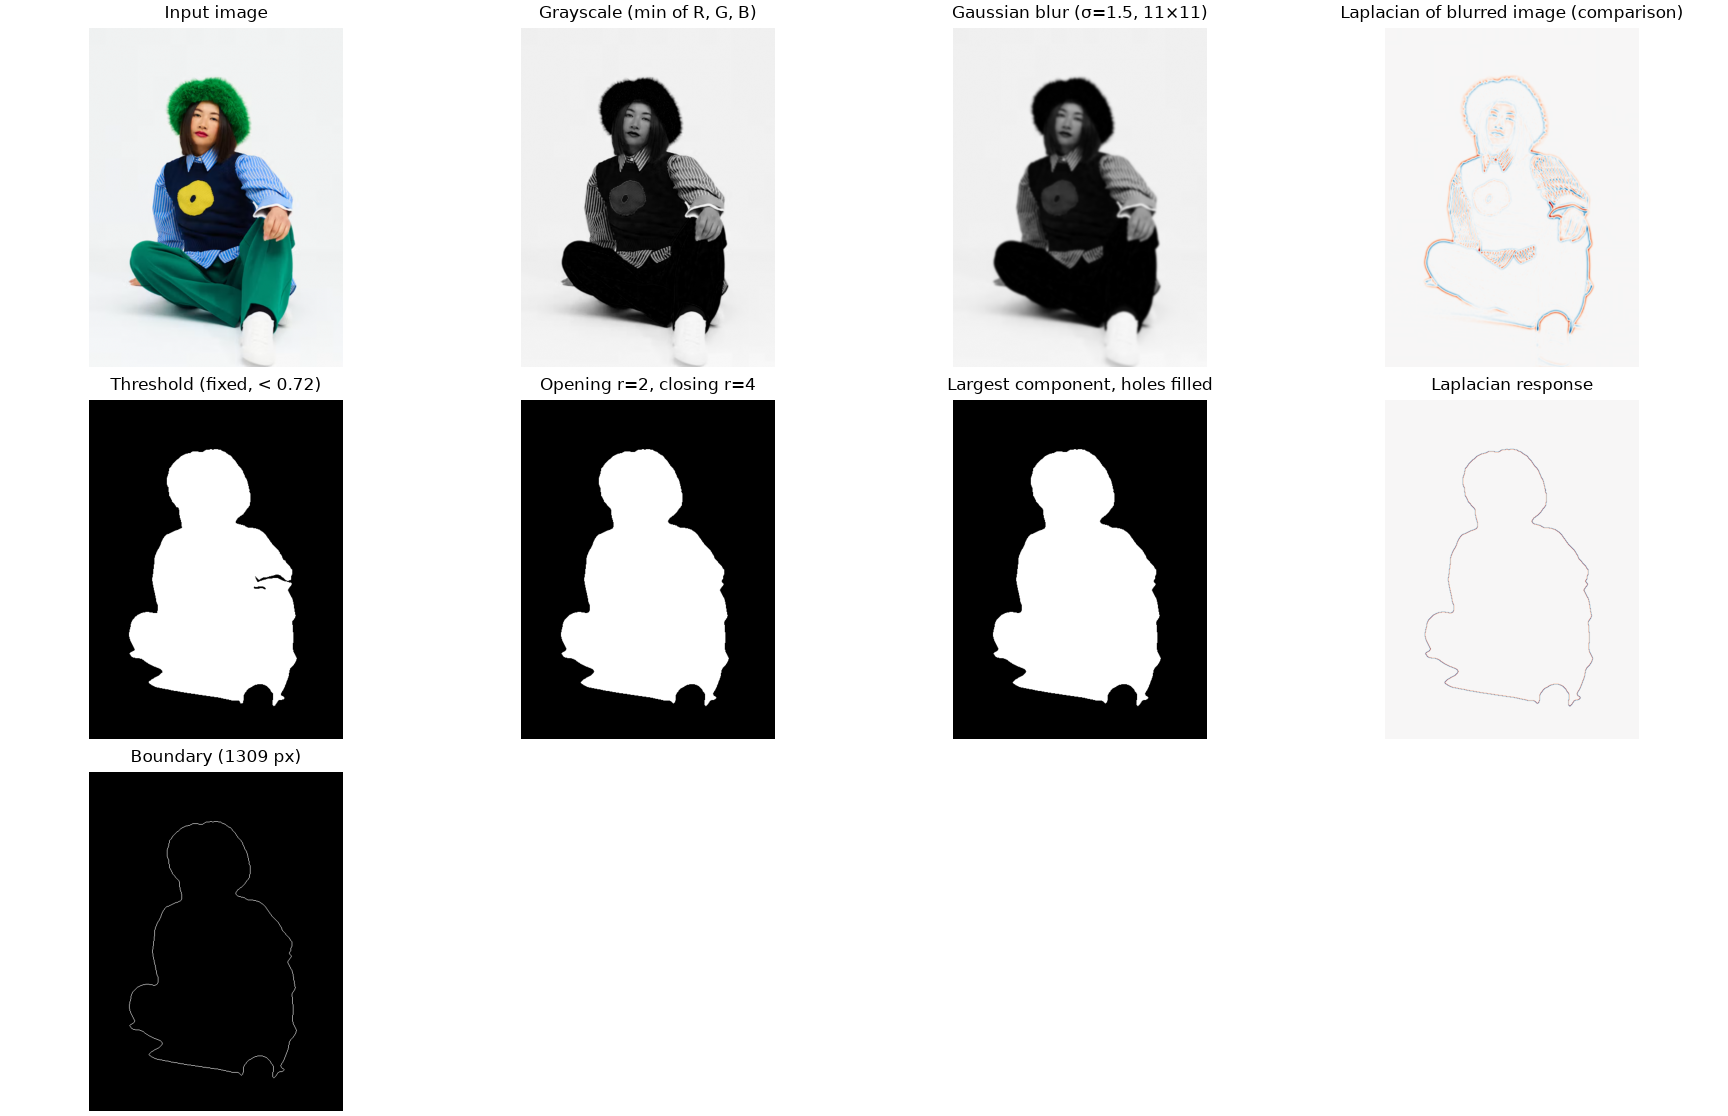
\includegraphics[width=0.5\linewidth]{assets/latex/03_transforms.png}
    \caption{Even with a middle-ground threshold, the girl's shadow is included in her outline while her shoe is excluded.}
    \label{fig:03_transforms}
\end{figure}

\subsection{Future Work}    

There are several improvements we could make that would address the shortcomings listed above. First, shadows use the same chroma value as the background, but at a lower intensity. A ratio would be able to reject this, removing the need for thresholds to account for shadows. This would improve performance on Image 03.

Second, using independent Fourier loops for multi-loop images would remove bridges between loops. While implementing this, the image-boundary issue should also be addressed. These fixes would improve the performance on any image with multiple loops, including Image 04. 

Finally, existing literature should be examined to explore automatic parameter setting. The biggest weakness of the implementation is its inability to generalise. Fixing this, giving it the ability to generate a viable output for any arbitrary input image, would make it a much more powerful project.

\section{Conclusion}

Overall, this has been an enjoyable and engaging project that has highlighted the power of Fourier transforms and let us explore techniques used in computer vision. We have learned how to break a signal into its constituent parts, how to use filters to improve the performance of image processing algorithms, and how to convert 2D data into a one dimensional signal. With more work, we could improve the effectiveness of the project, letting it generalise to a wider variety of images.

\end{document}
